\documentclass[a4paper]{article}
\usepackage[ngerman]{babel}
\usepackage[utf8]{inputenc}
\usepackage{multicol}
\usepackage{calc}
\usepackage{ifthen}
\usepackage[landscape]{geometry}
\usepackage{amsmath,amsthm,amsfonts,amssymb}
\usepackage{color,graphicx,overpic}
\usepackage{xcolor, listings}
\usepackage[compact]{titlesec} %less space for headers
\usepackage{mdwlist} %less space for lists
\usepackage{pdflscape}
\usepackage{verbatim}
\usepackage[most]{tcolorbox}
\usepackage[hidelinks,pdfencoding=auto]{hyperref}
\usepackage{bussproofs}
\usepackage{fancyhdr}
\usepackage{lastpage}
\pagestyle{fancy}
\fancyhf{}
\fancyhead[L]{Neurowissenschaften - Short}
\fancyfoot[L]{\thepage/\pageref{LastPage}}
\renewcommand{\headrulewidth}{0pt} %obere Trennlinie
\renewcommand{\footrulewidth}{0pt} %untere Trennlinie

\usepackage{pifont}
\newcommand{\cmark}{\ding{51}}
\newcommand{\xmark}{\ding{55}}

\pdfinfo{
 /Title (Neurowissenschaften - Short)
 /Creator (TeX)
 /Producer (pdfTeX 1.40.0)
 /Author (Robert Jeutter)
 /Subject ()
}
\geometry{top=1.3cm,left=1cm,right=1cm,bottom=1.2cm}

% Redefine section commands to use less space
\makeatletter
\renewcommand{\section}{\@startsection{section}{1}{0mm}%
 {-1ex plus -.5ex minus -.2ex}%
 {0.5ex plus .2ex}%x
 {\normalfont\large\bfseries}}
\renewcommand{\subsection}{\@startsection{subsection}{2}{0mm}%
 {-1explus -.5ex minus -.2ex}%
 {0.5ex plus .2ex}%
 {\normalfont\normalsize\bfseries}}
\renewcommand{\subsubsection}{\@startsection{subsubsection}{3}{0mm}%
 {-1ex plus -.5ex minus -.2ex}%
 {1ex plus .2ex}%
 {\normalfont\small\bfseries}}
\makeatother

% Don't print section numbers
\setcounter{secnumdepth}{0}
\setlength{\parindent}{0pt}
\setlength{\parskip}{0pt plus 0.5ex} 
% compress space
\setlength\abovedisplayskip{0pt}
\setlength{\parskip}{0pt}
\setlength{\parsep}{0pt}
\setlength{\topskip}{0pt}
\setlength{\topsep}{0pt}
\setlength{\partopsep}{0pt}
\linespread{0.5}
\titlespacing{\section}{0pt}{*0}{*0}
\titlespacing{\subsection}{0pt}{*0}{*0}
\titlespacing{\subsubsection}{0pt}{*0}{*0}

\begin{document}

\raggedright
\begin{multicols}{2}\scriptsize
    \begin{center}
        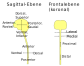
\includegraphics[width=.45\linewidth]{Assets/Neurowissenschaften-ebenen.png}
        \hspace{1cm}
        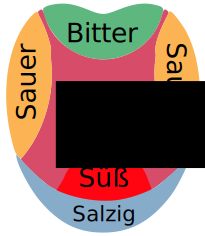
\includegraphics[width=.3\linewidth]{Assets/Neurowissenschaften-zunge.png}
    \end{center}

    \vspace{1cm}
    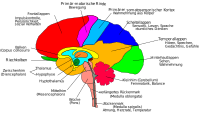
\includegraphics[width=\linewidth]{Assets/Neurowissenschaften-gehirn.png}

    \vspace{1cm}
    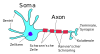
\includegraphics[width=\linewidth]{Assets/Neurowissenschaften-neuron.png}

    \vspace{1cm}
    \includegraphics[width=\linewidth]{Assets/Neurowissenschaften-rückenmark.png}

\end{multicols}
\end{document}